\documentclass{article}
\usepackage{delimset, diffcoeff, interval}
\usepackage[colorlinks=true, urlcolor=blue, linkcolor=blue, citecolor=blue]{hyperref}
\usepackage{amsmath, amsthm, amsfonts, mathtools, nicematrix, bm, cancel, siunitx}
\usepackage{subcaption}
\usepackage[linesnumbered,ruled,vlined]{algorithm2e}
\usepackage{graphicx, booktabs, accents, enumerate}
\usepackage{import, float, pdfpages, transparent, xcolor}
% \usepackage[a4paper, total={6in, 8in}]{geometry}
\usepackage[margin=1in]{geometry}
\usepackage[hang]{footmisc} % to make footnotes align
\usepackage{cleveref}
\usepackage{authblk}
\bibliographystyle{IEEEtran}
% \colorlinks=true
% \linkcolor=blue
% \urlcolor=cyan
% \documentstyle[fullpage]{article}
% Define theorem styles here based on the definition style (used for definitions and examples)
\theoremstyle{definition}
\newtheorem{definition}{Definition}
\newtheorem{claim}{Claim}
\newtheorem{implementation}{Implementation}
% Define theorem styles here based on the plain style (used for theorems, lemmas, propositions)
\theoremstyle{plain}
\newtheorem{theorem}{Theorem}[section]
\newtheorem{corollary}[theorem]{Corollary}
\newtheorem{lemma}[theorem]{Lemma}
\newtheorem{proposition}[theorem]{Proposition}
% Define theorem styles here based on the remark style (used for remarks and notes)
\theoremstyle{remark}
\newtheorem{example}[theorem]{Example}
\newtheorem*{warning}{Warning}
\newtheorem*{notation}{Notation}
\newtheorem{remark}[theorem]{Remark}
\newtheorem*{solution}{Solution}

% config
\intervalconfig{soft  open  fences ,separator  symbol=;,}

\newcommand\numberthis{\addtocounter{equation}{1}\tag{\theequation}} % so we can tag the final equation in a list of aligns
\newcommand{\defn}{\coloneqq} %defined as
\newcommand{\reals}{\mathbb{R}} %space of reals
\newcommand{\natrl}{\mathbb{N}} %space of natural numbers
\newcommand{\lap}{\Delta} %laplacian
\newcommand{\eps}{\epsilon}
\newcommand{\man}{\mathcal{M}} % manifold
\newcommand{\vg}{\dot{\gamma}} % dotted velocity curve
\newcommand{\veta}{\dot{\eta}} % dotted velocity eta
\newcommand{\tanb}{\Gamma T \man} % tangent bundle
\newcommand{\ddx}[1]{\diffp*{}{x^#1}}
% \DeclareMathOperator{\min}{min}
\DeclareMathOperator{\Tr}{Tr}

% To italicizse and bold rows in a table
\newcolumntype{+}{>{\global\let\currentrowstyle\relax}}
\newcolumntype{^}{>{\currentrowstyle}}
\newcommand{\rowstyle}[1]{\gdef\currentrowstyle{#1}%
#1\ignorespaces
}


\begin{document}
\title{Topological effects in gravitational lensing}
\author[1]{Alex Leviyev}
\affil[1]{Center for Graviational Physics, University of Texas at Austin}
\date{\today}
% \tableofcontents
\maketitle

\begin{abstract}
Deflection of light by gravitational fields is of significant practical interest in astrophysics. Applications range from constraining cosmological parameters to studying the distribution of dark matter in galaxies. In this note we review an interesting theoretical study illustrating that gravitational lensing depends on \textbf{topological} properties. That is, questions about whether multiple images appear, etc... may be answered by looking at topological properties of the spacetime. Global properties and curvature are related by the so called Gauss-Bonnet theorem, which relates the Gaussian curvature to the Euler characteristic.
% High-precision posterior exploration forms the backbone of many scientific and engineering disciplines, e.g astronomy. Popular tools used for such tasks are often based on the tried and true Metropolis-Hastings algorithm--a \textit{stochastic} procedure that simulates a Markov chain that is gauranteed to explore the target. However, simulating such a Markov chain for problems with computationally expensive physical models or large datasets is often infeasible. Stein variational gradient descent (SVGD) is an alternative that has recently blown up in popularity due to its tractability
\end{abstract}

% \section{Intro}
% \input{1-intro}
% \input{2-toyproblems}
% \input{extra}
% \appendix
%!TEX root = main.tex

\section{Introduction}

\begin{figure}[!htb]
	\centering
	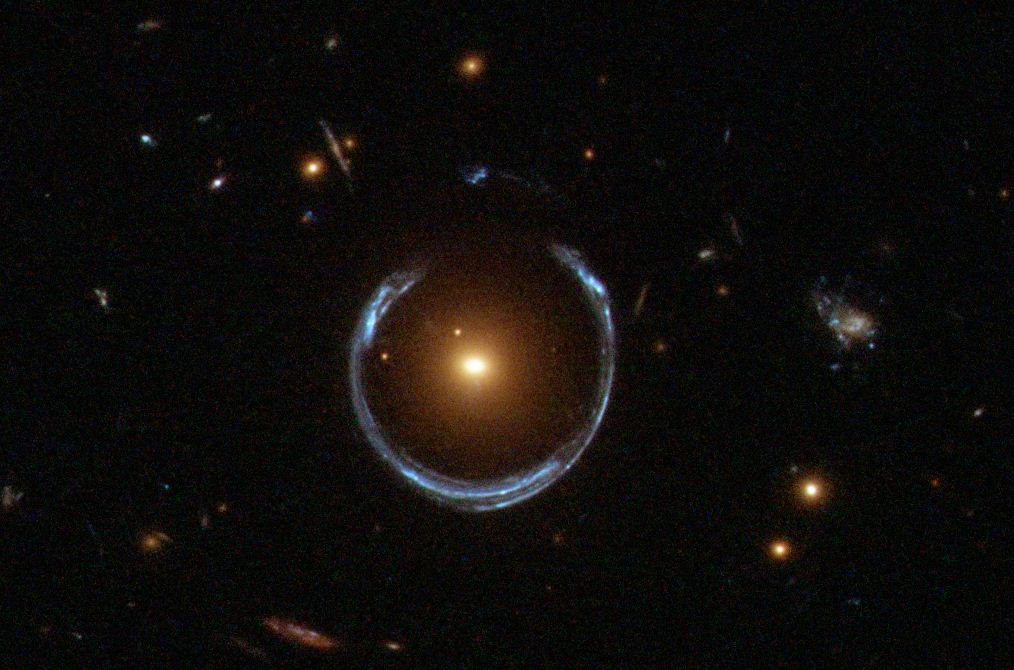
\includegraphics[width=0.65\textwidth]{img/einstein-ring.png}
	\caption{A so called ``Einstein ring". Source: \url{https://en.wikipedia.org/wiki/Gravitational_lens}}
	\label{}
\end{figure}

We will be discussing the phenomena of gravitational lensing using a relatively novel approach.
Although lensing is a inherently geometric phenomena, many lensing effects may be adequately studied in a Newtonian limit, and thus bypass the need to do general relativistic calculations.
This is not always the case however, and a lot of work has been done studying gravitational lensing in general Lorentzian manifolds \cite{1992grle.book.....S}.
The approach we follow here is a sort of middle ground, known as \textbf{optical geometry}, which replaces the problem of studying null geodesics (light rays) on a Lorentzian manifold $(\man, g)$ with studying geodesics of a simpler, purely spatial manifold $(\Sigma, \fermat)$.
This allows us to bring to bear all the powerful tools of classical surface analysis, and turns the study of the behavior of light rays in the presence of mass into a classical differential geometry problem!

We organize this note as follows.
We begin by briefly reviewing the generalization of Fermat's principle to Lorentzian spacetimes.
This generalization will lead to the observation that there exists a one to one correspondence between null geodesics on a static spacetime $(\man, g)$ and classical geodesics of a related spatial manifold $(\Sigma, \fermat)$, where $\fermat$ is called the \textbf{Fermat}, or \textbf{optical} metric.
The majority of the paper will be focused on studying the optical metric associated to the Schwarzschild metric.
Finally, we will show that gravitational lensing in a Schwarzschild spacetime occurs \textit{because} Schwarzschild has nontrivial genus (i.e, $g \ge 1$).\footnote{All of these concepts will be concretely defined in what follows.}

% This is the subject of \textbf{optical geometry}.
% We will begin by discussing the generalisation of Fermats principle to spacetime. In order to do concrete (optical geometric) calculations, we will specialize to \textbf{static spacetimes}, which turn out to have Riemannian structure.
% In this framework, we will see that gravitational lensing is a global effect, where the topology will determine whether we can have multiple images, what the deflection angles are, etc... This will utilize the so called Gauss Bonnet theorem.

\section{The optical geometry method}
\subsection{Fermat's principle}
Herod (10-75CE) postulated that light takes the shortest path between two points.
This appears to be the first version of \textbf{Fermat's principle}, which turns out to be correct for homogeneous media.
Generally, light always takes the shortest path \textit{in time}.
This may be posed as a calculus of variations problem in $\reals^3$ as follows.
Let $\gamma: (0,1) \to \reals^3$.
The actual path $\gamma$ taken extremizes the action $S[\gamma] \defn \int_{\gamma} \, dt = \frac{1}{c}\int_{\gamma} n \, dl$, where $n$ is a spatially varying refractive index, and $l$ is the arclength of the curve.
This is in regular Euclidean space however, we need a generalization of this principle to Lorentzian spacetimes.
%
% Recall the following definitions in the spacetime setting
%
% \begin{definition}[]\label{}
% Let $\gamma: I \to \man$ be a curve. Then $\gamma$ is a \textbf{null curve} if $g(\dot{\gamma}(\lambda), \dot{\gamma}(\lambda))=0$ for every $\lambda \in I$.
% \end{definition}
%
% \begin{definition}[]\label{}
% Let $\gamma: I \to \man$ be a curve. Then $\gamma$ is a \textbf{null geodesic} if it is a null curve, and $\nabla_{\dot{\gamma}} \dot{\gamma}$
% \end{definition}
%
% The distinction between null curves and null geodesics is of practical importance. A null geodesic satisfies the geodesic equations, implying that it is affinely parameterized. Loosely speaking, this means that the curve has constant velocity, and thus zero acceleration. This need not be the case for null curves.
%%%%%%%%%%%%%%%%%%%%%%%%%%%%%%%%%
%
%%%%%%%%%%%%%%%%%%%%%%%%%%%%%%%%%
% We introduce some notation and a result that will make our following calculations more transparent.
% \begin{definition}[]\label{}
% Let $\gamma: I \to \man$ be a curve. Then the \textbf{$i$'th coordinate image of $\gamma$ under $x$} is a map $\gamma^i_{(x)}: \reals \to \reals$ defined by
% \begin{equation}\label{}
% \gamma^i_{(x)}(\lambda) \defn (x \circ \gamma)^i (\lambda) = (x_i \circ \gamma) (\lambda)
% \end{equation}
% \end{definition}
%
% \begin{definition}[]\label{}
% Let $\gamma: I \to \man$ be a curve. Then the \textbf{velocity field along $\gamma$} is the map $\vg: \reals \to \tanb$ such that $\lambda \mapsto \vg_{(x)}^i (\lambda) \ddx{i} \rvert_{\gamma(\lambda)}$
% \end{definition}
%
% \begin{remark}[]\label{}
% Note that the components of the velocities are the derivatives of the curve image components.
% \end{remark}
% \begin{proposition}[]\label{}
% Let $\gamma: I \to \man$ be a curve, and $\vg$ be the velocity field along $\gamma$. Then
% \begin{equation}\label{}
% g(\vg(\lambda), \vg(\lambda)) = \vg_{(x)}^{\mu}(\lambda) \vg_{(x)}^{\nu}(\lambda) g_{\mu \nu} \rvert_{\gamma(\lambda)}
% \end{equation}
% \end{proposition}
% \begin{proof}
% \begin{align*}
% g(\vg(\lam), \vg(\lam)) &= g(\vg_{(x)}^{\mu} (\lam) \diffp{}{x^{\mu}}, \vg_{(x)}^{\nu} (\lam) \diffp{}{x^{\nu}}) \\
% &=\vg_{(x)}^{\mu} (\lam)\vg_{(x)}^{\nu} (\lam)g( \diffp{}{x^{\mu}},  \diffp{}{x^{\nu}})\\
% &= \vg_{(x)}^{\mu} (\lam)\vg_{(x)}^{\nu} (\lam)g_{\mu \nu} \at_{\gam(\lam)}
% \end{align*}
% \end{proof}
%
Before stating the generalization of Fermat's principle to spacetime, we introduce the following definition from the calculus of variations on smooth manifolds which will be used in the proof (and later when we discuss geodesic deviation).\footnote{We only need the statement of the theorem in what follows, but the proof is presented as well due to its simplicity.}
\begin{definition}[]\label{def:variation}
Let $\gamma: I \to \man$ be a smooth curve on a smooth manifold $(\man, g)$. A \textbf{variation} of $\gamma$ is a smooth function $\phi: (-\eps, \eps) \times I \to \man$ (for some $\eps>0$) such that $\gamma(t) = \phi(0, t) \; \forall t \in I$. For each fixed $s\in (-\eps, \eps)$, the path $\gamma_s(t) \defn \phi(s, t)$ is called a \textbf{curve of the variation}, and the vector field along $\gamma$ defined by $w(t) \defn \nabla_s \phi(0, t)$ is called the \textbf{variational vector field} of $\phi$. The variation $\phi$ is called \textbf{orthogonal} if $g(w(t), \gamma'(t))$ $\; \forall t \in I$.
\end{definition}
In contrast to the classical Fermat principle on $\reals^3$, which chooses a path which extremizes the total journey time (a global quantity), on spacetime Fermat's principle chooses the path which extremizes the \textit{arrival time} of a light ray (a local property). See \cref{fig:fermat-spacetime} for the setup.
\begin{theorem}[Fermat \cite{1992grle.book.....S}]\label{}
Let $(\man, g)$ be a spacetime, $S \in \man$ be a source, and $l$ be an observer. Then a smooth null curve $\gamma: (0,1) \to \man$ such that $\gamma(0) = S$ and $\gamma(1) = l(\tau)$ is a null geodesic iff its arrival time functional $\tau[\gamma]$ is stationary under first order variations of $\gamma$ within the set of smooth null curves from $S$ to $l$.
\end{theorem}
\begin{proof}
$(\implies)$. Consider a family of variances $\eta(\lambda, \epsilon)$ such that $\eta(\cdot, \epsilon) : (0,1) \to \man$, $\eta(0, \epsilon) = S$ for every $\eps \le \abs{\eps_0} \ll 1$, and $\eta(1, \epsilon) = l(\tau_0 + t(\epsilon))$ where $t: \reals \to \reals$ with $t(0)=0$.
Furthermore, let $g(\veta(\lambda, \eps), \veta(\lambda, \eps)) = 0$ for every $\lambda \in (0,1)$, where $\veta$ denotes the velocity field along $\eta(\cdot, \eps)$. We have constructed a family of null variations with fixed beginning and open end.
%
\begin{figure}[!htb]
	\centering
	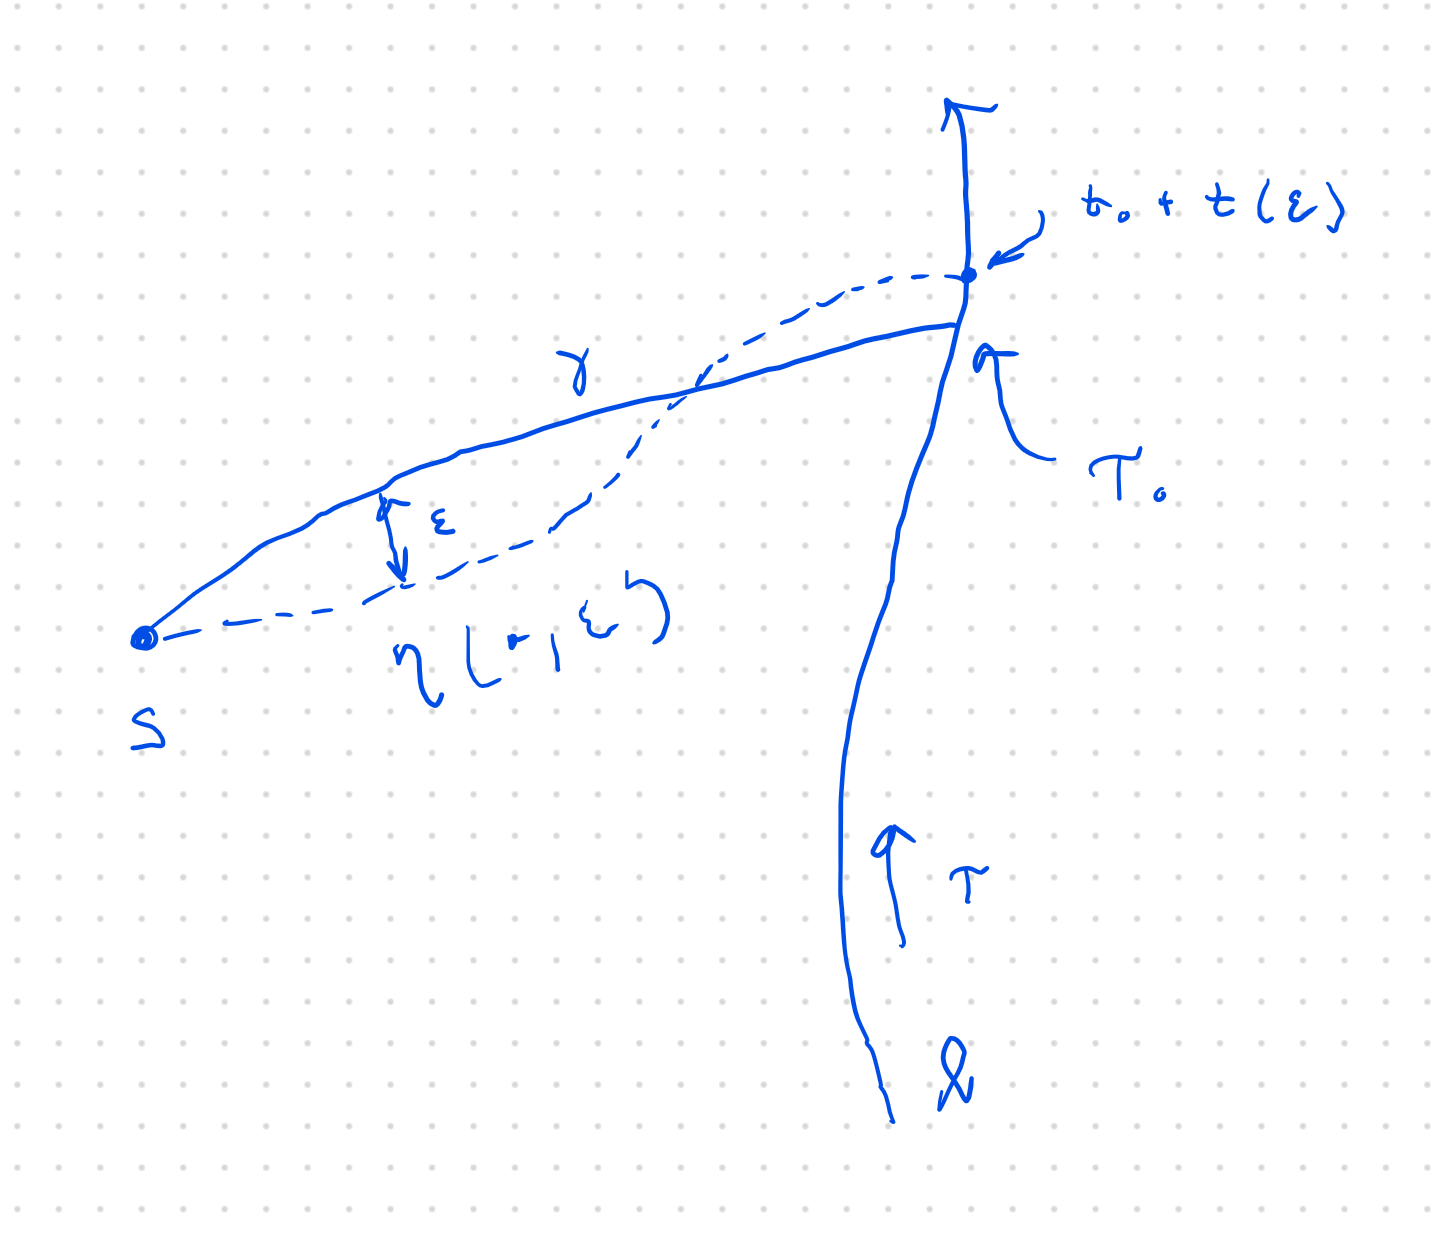
\includegraphics[width=0.5\textwidth]{img/null-variations.png}
	\caption{Illustration of Fermat's principle on spacetime. $\eta$ represents a variation for which every curve of the variation is a null curve. $l$ denotes an observer. The arrival time functional $\tau[\eta_{\eps}]$ (which crucially depends on the path chosen) is extremized.}
	\label{fig:fermat-spacetime}
\end{figure}

The action takes the form
\begin{equation}\label{}
S[\gamma_{\eps}] = \int_0^1 L(\eta(\lambda, \eps), \nabla_{\lam} \eta(\lam, \eps)) \, d\lam
\end{equation}
with the Lagrangian
\begin{align*}
L(\eta(\lam, \eps), \veta(\lam, \eps)) &= \frac{1}{2} g (\nabla_{\lam} \eta(\lam, \eps), \nabla_{\lam} \eta(\lam, \eps)) \\
&= \frac{1}{2} g_{\mu, \nu} \rvert_{\gamma(\lam)} \veta^{\mu} (\lam, \eps) \veta^{\nu}(\lam, \eps)
\end{align*}
%
We now differentiate
\begin{align*}
\diff{}{\eps} \frac{1}{2} \int_0^1 g_{\mu \nu} \at_{\gamma(\lam)} \veta^{\mu}(\lam, \eps) \veta^{\nu}(\lam, \eps) \, d\lam
&= \int_0^1 g_{\mu \nu} \at_{\gamma(\lam)} \diff{}{\eps}\brk[s]!{\veta^{\mu}(\lam, \eps)} \veta^{\nu}(\lam, \eps) \, d\lam \\
&= \int_0^1 \veta_{\mu} (\lam, \eps) \diff{}{\eps} \brk[s]!{\veta^{\mu} (\lam, \eps)} \, d\lam
= \int_0^1 \veta_{\mu} (\lam, \eps) \diff{}{\lam} \diff{}{\eps} \eta^{\mu} (\lam, \eps) \, d\lam\\
&= - \int_0^1 \ddot{\eta_{\mu}}(\lam, \eps) \brk[s]!{\diff{}{\eps} \eta^{\mu}(\lam, \eps)} \, d\lam + \brk[s]!{\veta_{\mu} (\lam, \eps) \diff{}{\eps} \brk[r]1{\eta^{\mu}(\lam, \eps)}}^{\lam = 1}_{\lam=0}
\end{align*}
Recall that we have constructed our variation such that $\eta^{\mu}(\lam, \eps) = \xi^{\mu}(\tau_0 + t(\eps))$. Thus the first term simplifies to
\begin{equation}\label{}
-\int_0^1 \ddot{\eta}_{\mu}(\lam, \eps) \dot{\xi}^{\mu}(\tau_0 + t(\eps)) \cdot \dot{t}(\eps) \, d\lam \at_{\eps=0} =
-\int_0^1 \ddot{\gamma}_{\mu}(\lam) \dot{\xi}^{\mu}(\tau_0) \cdot \dot{t}(0) \, d\lam \at_{\eps=0} = 0
\end{equation}
where the last equality is true because $\gamma$ is a geodesic, and therefore must have a affine parameterization (constant speed). The second term yields
\begin{align*}
\brk[s]1{\veta_{\mu} (\lam, \eps) \diff{}{\eps} (\eta^{\mu}(\lam, \eps))}^{\lam = 1}_{\lam = 0}
&= \veta_{\mu} (1, \eps) \diff{}{\eps} (\eta^{\mu}(1, \eps))
-  \veta_{\mu} (0, \eps) \diff{}{\eps} (\eta^{\mu}(0, \eps)) \\
&=\veta_{\mu} (1, \eps) \diff{}{\eps} (\xi^{\mu}(\tau_0 + t(\eps)) \\
&=\veta_{\mu} (1, \eps) \diff{}{\eps} (\dot{\xi}^{\mu}(\tau_0 + t(\eps)) \dot{t}(\eps) \\
&\implies \veta_{\mu} (1, 0) \diff{}{0} (\dot{\xi}^{\mu}(\tau_0 + t(0)) \dot{t}(0)
\end{align*}
Since $\veta$ is lightlike and $\dot{\xi}$ is timelike, their contraction is nonzero. This implies that $\dot{t}(0)$.
%
\\$(\impliedby)$ See \cite{1992grle.book.....S}.
\end{proof}
%

\subsection{From Lorentzian manifold to spatial manifold}
A well known feature of general relativity is that light rays follow null geodesics in spacetime.
Interestingly, we may show using Fermat's theorem \cite{PerlickV1990OFpi} that null geodesics on a \textbf{stationary} spacetime are in one-to-one correspondence with geodesics on a Finsler-Randers type manifold\footnote{This class of metric was initially proposed as an alternative model of gravity which features a preferred direction for time. Although the generalizations are straightforward, we will only investigate Riemannian metrics in what follows. Note that Finsler-Randers metrics contain Riemannian metrics as a special case.}, and null geodesics on a \textbf{static} spacetime are in one-to-one correspondence with geodesics on a Riemannian manifold. The strategy of optical geometry is to study these simpler spatial geodesics instead. These simpler metrics are called the \textbf{optical metric}, or the \textbf{Fermat metric}.

\begin{definition}[]\label{}
A spacetime $(\man, g)$ is called \textbf{stationary} if there is a timelike killing vector field $T \in \tanb$ satisfying
%
\begin{enumerate}[i)]
  \item $g(T, T) = 0$
  \item $\lie_Tg = 0$
\end{enumerate}
\end{definition}
%
Although this formalism works for stationary spacetimes, we will restrict ourselves to the following special case.
%
\begin{definition}[]\label{}
A spacetime $(\man, g)$ is called \textbf{static} if it is stationary, and its timelike Killing vector field $T$ is \textbf{hypersurface orthogonal}. That is, $T_{[a} \partial_b T_{c]} = 0$.
\end{definition}
\begin{remark}[Static spacetimes]\label{}
It may be shown \cite{straumann2012general} that there exist coordinates for a static spacetime such that the metric decomposes to
\begin{equation}\label{eq:static-metric-def}
g = -V^2 dt^2 + h_{ab} dx^a dx^b
\end{equation}
where $V^2 \defn T^a T_a$, and $h_{ab}$ has $(+, +, +)$ signature.
Furthermore, the null geodesics of a Lorentzian metric are unaffected by \textbf{conformal transformations} of the metric. That is, multiplication by positive functions. Since we are interested only in light rays, we may divide the RHS of \cref{eq:static-metric-def} by $V^2$ without loss of generality, and consider instead
\begin{equation}\label{eq:static-metric}
g = -dt^2 + \fermat_{ab} dx^a dx^b
\end{equation}
where $\fermat_{ab} \defn \frac{h_{ab}}{V^2}$.
\end{remark}
\begin{corollary}[]\label{}
The null geodesics on a static spacetime with metric given by \cref{eq:static-metric} are equivalent to the geodesics of a Riemannian manifold with metric $\fermat$.
\end{corollary}
\begin{proof}
Let $\eta$ be a null curve, and consider the proof of Fermat's principle from earlier. Let us consider the special case where the observer is an integral curve of the Killing vector $T$, such that
\begin{equation}\label{}
l^{\mu} = (\lambda, x_1, x_2, x_3)
\end{equation}
The fact that $\eta$ must be a null curve provides a relationship between its derivative components
\begin{equation}\label{}
\dot{\eta}^0 = \sqrt{\fermat_{ij} \dot{\eta}^i \dot{\eta}^j}
\end{equation}
We know that $\eta^0(0) = const$, $\eta^0(1) = \tau(\eta)$. Therefore
\begin{align*}
\int_0^1 \dot{\eta}^0 &= \dot{\eta}^0(1) - \dot{\eta}^0(0) = \int_0^1 \sqrt{\fermat_{ij} \dot{\eta}^i \dot{\eta}^j} \\
&\implies \tau(\eta) = \int_0^1 \sqrt{\fermat_{ij} \dot{\eta}^i \dot{\eta}^j} ds + const
\end{align*}
Note that since static metrics have time independent components, the RHS is independent of time, and resembles the length functional on a Riemannian manifold with metric $h$. By Fermat's theorem, varying this length functional will return a null geodesic of the original spacetime.
\end{proof}

%
% Using this definition we may obtain constraints on what a stationary metric must look like in coordinates. First, we have the following result.
% \begin{corollary}[]\label{}
% Suppose $(\man, g)$ is a stationary spacetime. Then there exists a chart for which components of the metric are time independent.
% \end{corollary}
% \begin{proof}
% Suppose we pick a chart such that the vector field $T$ may be expressed as $T = \delta^{\mu}_0 \diffp{}{x^{\mu}}$. Thus
% \begin{align*}
% (\lie_T g)_{\mu \nu} &= T^{\lam} g_{\mu \nu, \lam} + g_{\lam \nu} T^{\lam}_{,\mu} + g_{\mu \lam} T^{\lam}_{,\nu} = g_{\mu \nu, 0} = 0
% \end{align*}
% \end{proof}
%
% We may now write down the most general spacetime satisfying this property
% %
% \begin{equation}\label{}
% g = g_{\mu \nu} dx^{\mu} \otimes dx^{\nu} = -V^2(dt + \omega_a dx^a)^{\otimes 2} + h_{ab} dx^a \otimes dx^b
% \end{equation}
% %
% where $V$ is a positive function representing the norm of the Killing field, $h_{ab}$ form the components of a Riemann metric, and $\omega_a$ is the 3-vector called the \textbf{twist vector}, which measures the extent to which $T$ fails to be orthogonal to a family of three surfaces. Such a metric is known as a \textbf{Finsler-Randers} metric.
% In matrix form, the components of the metric take the form:
% $$
% [g_{\mu \nu}] =
% \begin{pNiceArray}{C|C}
% -V^2 & -v^2 \omega^{\top} \\
% \hline
% -V^2 \omega & h \\
% \end{pNiceArray}
% $$
% \begin{definition}[]\label{}
% A spacetime $(\man, g)$ is called \textbf{static} if it is stationary, and the twisting vector is zero.
% \end{definition}

\section{Optical geometry of Schwarzschild}
In this section we use the correspondence just established to study the optical geometry of the Schwarzschild metric, which we will see yields a two-dimensional Riemannian metric (\cref{def:schwarz-fermat}).
A natural question to ask when one receives a two-dimensional Riemannian manifold is ``can I visualize this two-manifold as an embedded surface in three dimensional Euclidean space?"
The answer in this case is yes, and turns out to be simpler than one may think at first glance: finding an explicit embedding is unnecessary.
Instead, we find a relationship for the derivatives of the surface parameterized in cylindrical coordinates (\cref{prop:derivatives-embed}), which will allow us to visualize the optical geometry in Euclidean space $\euc$ .
We will see that this embedded surface has a ``catenoid" like shape (\cref{fig:embedding}) which yields an everywhere negative Gaussian curvature (\cref{prop:neg-gauss-curve}).

\begin{definition}[]\label{}
The components of the \textbf{Schwarzschild metric} are given by
\begin{equation}\label{}
g = -\brk[r]2{1-\frac{2m}{r}} dt^2 + \frac{dr^2}{1-\frac{2m}{r}} + r^2(d\theta^2 + sin^2\theta d\phi^2)
\end{equation}

\end{definition}

Without loss of generality we only consider the equatorial plane $\theta=\frac{\pi}{2}$.
\begin{definition}[]\label{def:schwarz-fermat}
The components of the \textbf{optical metric of equatorial Schwarzschild} are given by
\begin{equation}\label{}
\fermat = \frac{dr^2}{\brk[r]1{1 - \frac{2m}{r}}^2} + \frac{r^2}{1 - \frac{2m}{r}} d\phi^2.
\end{equation}
The geodesics of this metric are called \textbf{spatial light rays}.
\end{definition}

\subsection{Visualizing the optical geometry of Schwarzschild}
To build intuition for this geometry we aim to find an isometric embedding into three dimensional Euclidean space $\mathbb{E}^3$. We proceed in cylindrical coordinates
% \begin{equation}\label{}
% dt^2 = \frac{dr^2}{\brk[r]1{1 - \frac{2m}{r}}^2} + \frac{r^2}{1 - \frac{2m}{r}} d\phi^2
% \end{equation}
\begin{align*}
\fermat &= \frac{dr^2}{\brk[r]1{1 - \frac{2m}{r}}^2} + \frac{r^2}{1 - \frac{2m}{r}} d\phi^2 = dz^2 + dR^2 + R^2 d\phi^2.
\end{align*}
The following result will help us visualize this surface.
%
\begin{proposition}[]\label{prop:derivatives-embed}
Let $(z, R, \phi)$ denote cylindrical coordinates. Then for the optical metric of equatorial Schwarzschild the following holds:
\begin{equation}\label{}
\diff{z}{R} = \frac{\sqrt{4mr-9m^2}}{r-3m}.
\end{equation}
\end{proposition}
%
\begin{proof}
The following will be used to simplify the algebra
\begin{align*}
f(r) &\defn \sqrt{1 - \frac{2m}{r}} \\
f'(r) &= \frac{1}{2}\brk[r]2{1-\frac{2m}{r}}^{-\frac{1}{2}}\frac{2m}{r^2} = \frac{m}{r^2f} \\
f^4 &= \brk[r]2{1 - \frac{2m}{r}}^2 = 1 + \frac{4m^2}{r^2} - \frac{4m}{r}
\end{align*}
Observe that $R(r) = \frac{r}{f}$. Likewise,
\begin{equation}\label{}
\diff{R}{r} = \diff{}{r} \brk[r]2{\frac{r}{f}} = \frac{f - rf'}{f^2} = f^{-1} - \frac{m}{rf^3} = \frac{rf^2 - m}{rf^3}
\end{equation}
We find an expression for $\diff{z}{R}$.
\begin{align*}
\frac{1}{f^4} + \frac{r^2}{f^2} \brk[r]2{\diff{\phi}{r}} &= \brk[r]2{\diff{z}{r}} + \brk[r]2{\diff{R}{r}} + R^2 \brk[r]2{\diff{\phi}{r}} \\
\implies \frac{1}{f^4} &= \brk[r]2{\diff{z}{r}}^2 + \brk[r]2{\diff{R}{r}}^2 = \brk[r]2{\diff{z}{R}}^2 \brk[r]2{\diff{R}{r}}^2 + \brk[r]2{\diff{R}{r}}^2 = \brk[s]2{\brk[r]2{\diff{z}{R}}^2 + 1}\brk[r]2{\diff{R}{r}}^2 \\
\implies \brk[r]2{\diff{z}{R}}^2 &= \frac{1}{f^4} \brk[r]2{\diff{R}{r}}^{-2} - 1 = \frac{r^2 f^6}{(rf^2 + m)^2} - 1 \\
\implies (rf^2-m)^2 &= r^2f^4 - 2rf^2m + m^2 \\
&= r^2 \brk[r]2{1 - \frac{2m}{r}^2} - 2r \brk[r]2{1 - \frac{2m}{r}}m + m^2 \\
&= r^2 \brk[r]2{1 - \frac{4m}{r} + \frac{4m^2}{r^2}} - 2rm + 4m^2 + m^2 \\
&= r^2 - 4mr + 4m^2 - 2rm + 4m^2 + m^2 \\
&= r^2 - 6mr + 9m^2 \\
\implies \brk[r]2{\diff{z}{R}}^2 &= \frac{r^2 \brk[r]2{1 - \frac{2m}{r}}}{r^2 - 6mr + 9m^2} + \frac{-r^2 + 6mr - 9m^2}{r^2 - 6mr + 9m^2} \\
&= \frac{4mr - 9m^2}{(r-3m)^2} \, ,
\end{align*}
which yields the desired result.
\end{proof}
In light of the previous calculation, we make the following observations:
\begin{enumerate}[i)]
\item The embedding is restricted to $4mr - 9m^2 > 0 \implies 4r > 9m \implies r > \frac{9}{4}m$ and therefore does not work for $2m < r < \frac{9}{4}m$.
\item Observe that asymptotically, $R \rightarrow r$. Hence
\begin{equation}\label{}
\lim_{r \uparrow \infty} \brk[r]2{\diff{z}{R}}^2 = \frac{4mR}{R^2} = \frac{4m}{R} \implies \diff{z}{R} = 2\sqrt{\frac{m}{R}}
\end{equation}
I.e, $z$ goes as $\sqrt{R}$ asymptotically
\item
$\diff{z}{R}$ is singular at $R(r=3m)$. This corresponds to the circular photon orbit of Schwarzschild.
\item
For $r>3m$, the slope is positive. On the other hand, for $\frac{9}{4}m < r < 3m$ the slope is negative.
\end{enumerate}
%
A surface with these properties is represented in \cref{fig:embedding}.
Visually, it appears as though this surface has everywhere negative Gaussian curvature. Indeed this is case, and may be shown analytically.
\begin{proposition}[]\label{prop:neg-gauss-curve}
The Gaussian curvature associated with the Fermat metric of equatorial Schwarzschild has everywhere negative curvature. Specifically, for $r > \frac{9}{4}m$,
\begin{equation}\label{}
K = - \frac{2m}{r^3}\brk[r]2{1 - \frac{3m}{2r}} < 0.
\end{equation}
\end{proposition}
%
\begin{figure}[!htb]
	\centering
	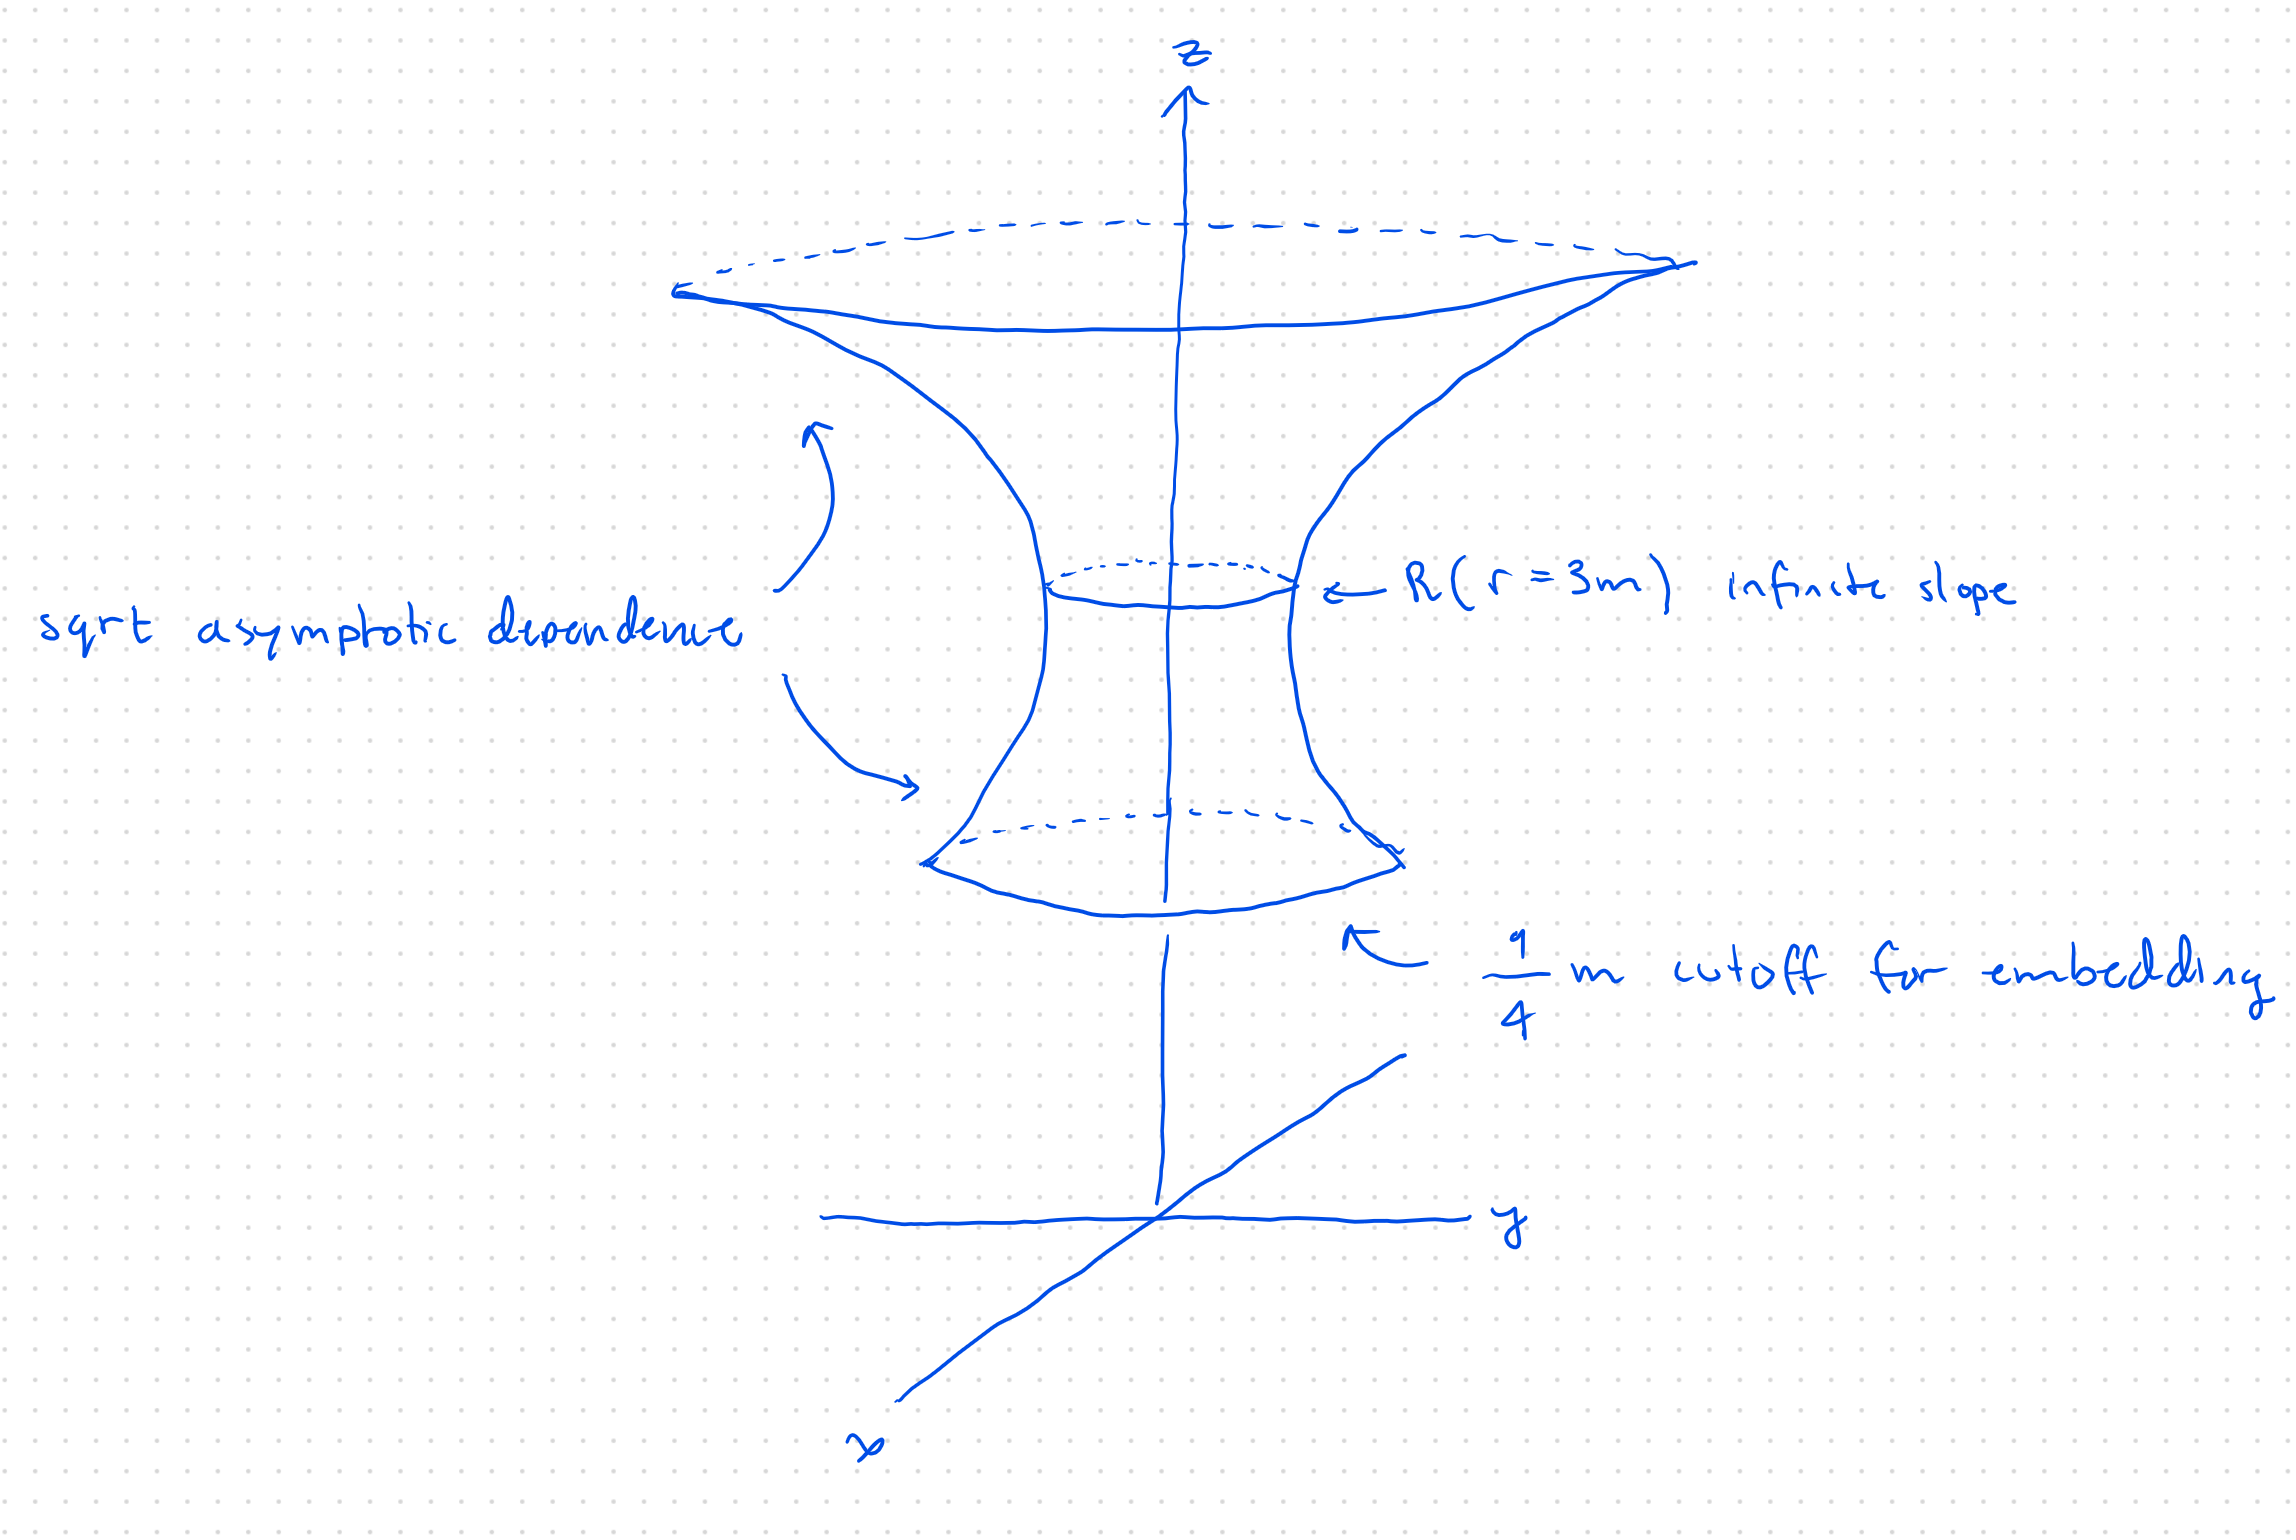
\includegraphics[width=0.95\textwidth]{img/embedding.png}
	\caption{The embedding in $\mathbb{E}$ of the equatorial Schwarzschild-Fermat metric.}
	\label{fig:embedding}
\end{figure}

% \section{Gauss-Bonnet and gravitational lensing}
We are now in possession of a negatively curved surface $\Sigma$ on which geodesic behavior tells us about the behavior of light rays on the equatorial plane of Schwarzschild. We may now use well known results from surface analysis to tease out the physics we are interested in.

\begin{figure}[!htb]
	\centering
	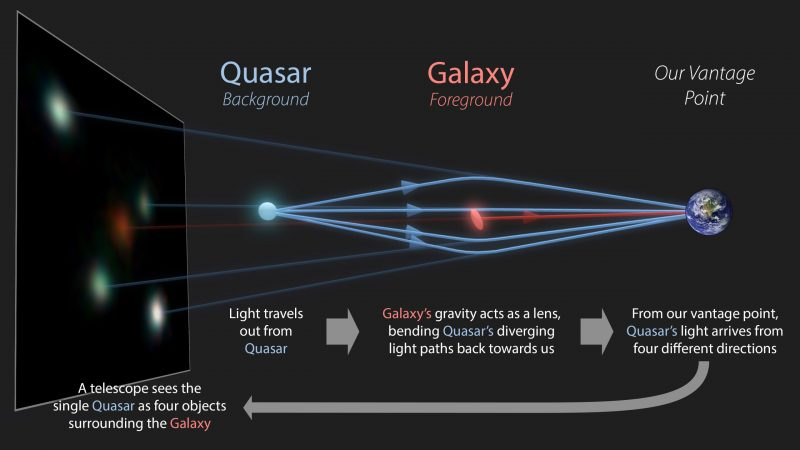
\includegraphics[width=0.7\textwidth]{img/lensing.png}
	\caption{An illustration of lensing. Mathematically, this is modelled by the intersection of the light ray with an observer. Source: \url{https://earthsky.org/space/what-is-gravitational-lensing-einstein-ring/}}
	\label{fig:lensing}
\end{figure}

\subsection{Geodesic deviation}
Note that gravitational lensing can only occur when two or more geodesics emanating from the same point $s \in \Sigma$ (source) on the catenoid recombine at a later point $o \in \Sigma$ (observer) as in \cref{fig:lensing}.
A fact of life however is that geodesics diverge locally in the presence of negative curvature (\cref{thm:geodesic-deviation}), which at face value seems to imply that geodesics never rejoin in a Schwarzschild spacetime.
However, it turns out that geodesics may rejoin even on a surface with negative curvature as long as the surface is not \textit{simply connected}.
Indeed this is the case for the optical geometry (\cref{thm:nontrivial-topology}), and in this way a nontrivial topology allows for gravitational lensing to occur.

% \begin{question}[]\label{}
% Under what circumstances can two geodesics with the same initial point $s \in \Sigma$ (source) meet at another point $o \in \Sigma$ (observer)?

% \end{question}
Before moving forward, we discuss some of the tools we will need to make sense of negatively curved surfaces. Specifically, to show that geodesics locally diverge in the presence of negative curvature requires the concept of \textit{Jacobi fields}, which provide the appropriate ``data structure" to work with when we are interested in studying the behavior of geodesics nearby a ``reference" geodesic.
\begin{definition}[]\label{}
Let $\Sigma$ be a regular surface and $\gamma: I \to \Sigma$ be a geodesic. A variation of $\gamma$ is called a \textbf{geodesic variation} if every curve of the variation is a geodesic.
\end{definition}
\begin{definition}[]\label{}
Let $\gamma: I \to \Sigma$ be a geodesic on a regular surface $\Sigma$. A vector field $J$ along $\gamma$ is said to be a \textbf{Jacobi field} if it satisfies the \textbf{Jacobi equation}
\begin{equation}\label{}
\nabla^2_t J = -K(\Sigma) J \, ,
\end{equation}
for every $t \in I$. Here $K(\Sigma)$ denotes the Gaussian curvature of $\Sigma$.
\end{definition}
\begin{proposition}[]\label{}
Let $\gamma: I \to \Sigma$ be a geodesic parameterized by arclength on a regular surface $\Sigma$. Then the variational vector field of (any) geodesic variation of $\gamma$ is a Jacobi field. Conversely, given $\gamma$ and a Jacobi field $J$ along $\gamma$, one may extend $\gamma$ to a geodesic variation.
\end{proposition}
%
The norm of the Jacobi field controls the ``rate of spread" of nearby geodesics. The next result is a Taylor expansion of the norm of the Jacobi field along $\gamma$, and shows that the rate of spread ``feels" curvature beginning at third order.
%
\begin{theorem}[]\label{thm:geodesic-deviation}
Let $\gamma: I \to \Sigma$ be a curve in $\Sigma$ such that $\gamma(0)=p$, $\dot{\gamma}(0) = v$. Now, let $J$ be a Jacobi field along $\gamma$ satisfying $J(0)=0$, $J'(0)=w$, and suppose $g(v,v)=g(w,w)=1$. Then
\begin{equation}\label{}
\norm{J(t)} = t - \frac{K}{6}t^3 + \order(t^4)
\end{equation}
where $K$ is the Gaussian curvature of $\Sigma$.
\end{theorem}
\begin{figure}[!htb]
	\centering
	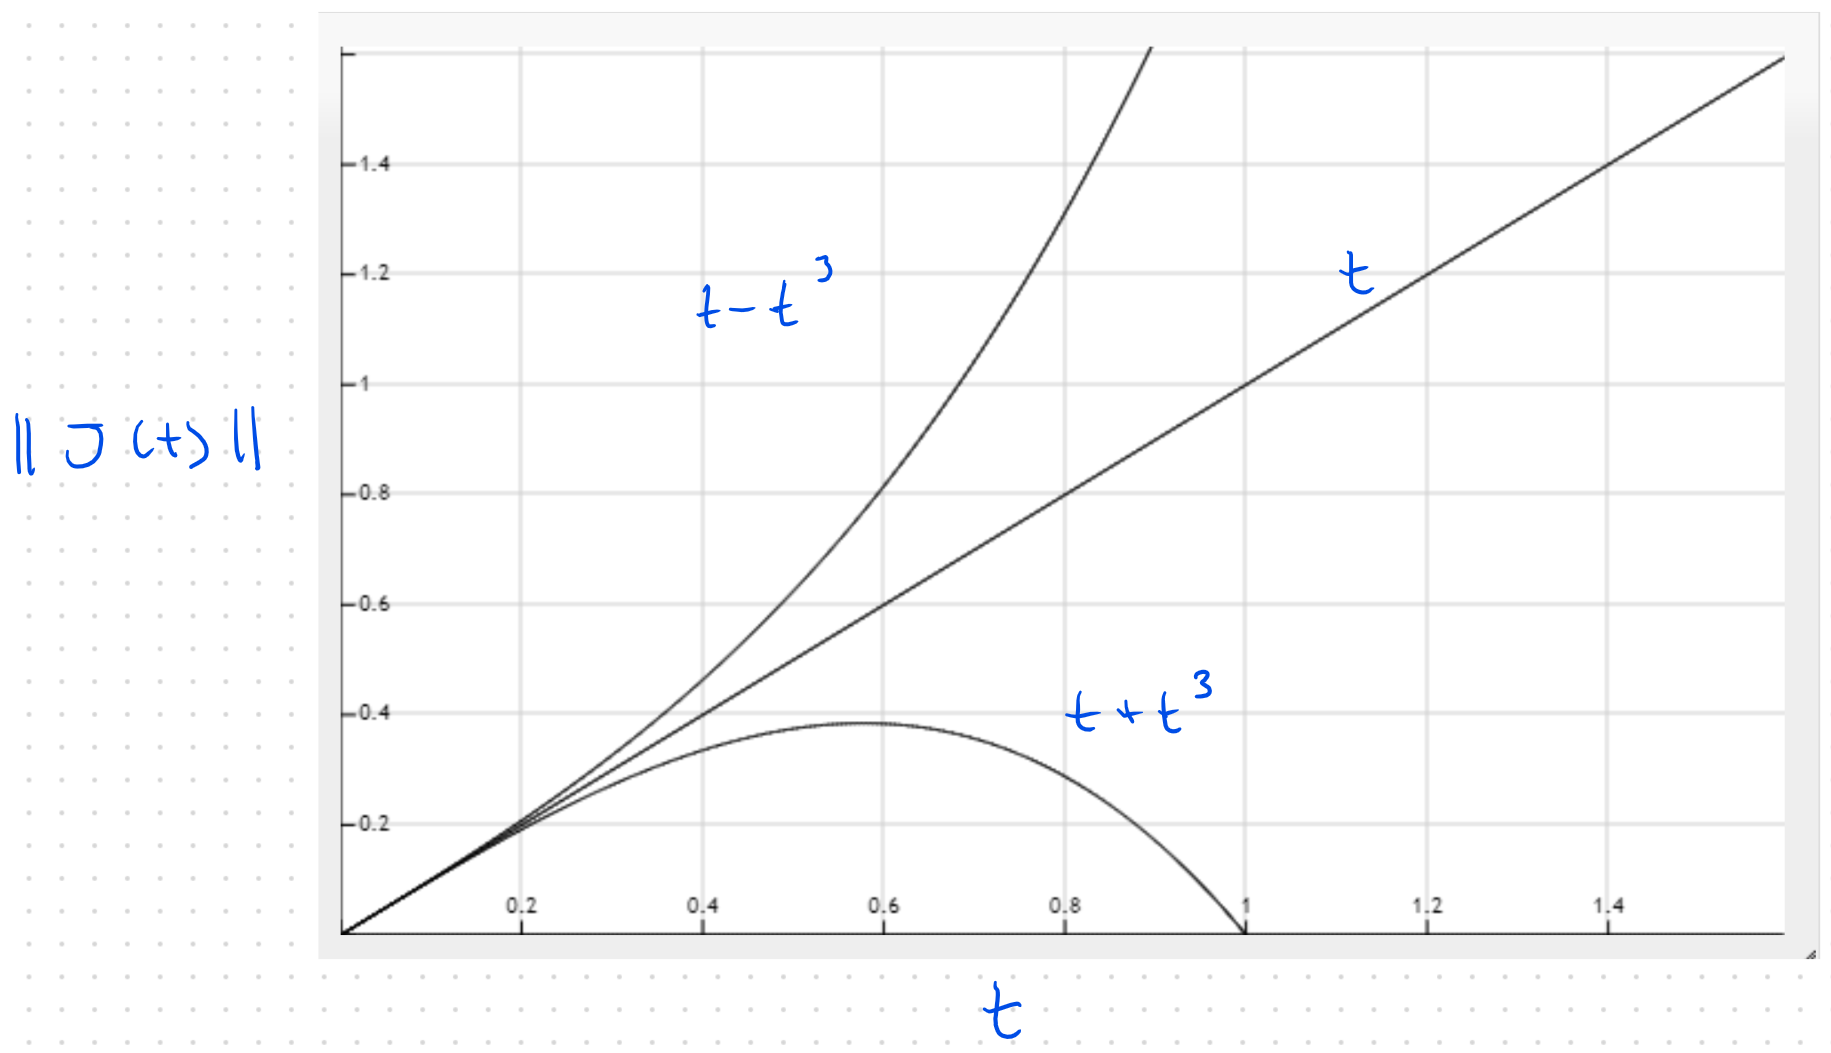
\includegraphics[width=0.7\textwidth]{img/deviation.png}
	\caption{An illustration of the effect that curvature has on geodesic deviation. The straight line shows how straight lines would deviate from each other in flat space. The presense of negative or positive curvature cause a ``deviation" from flat space.}
	\label{}
\end{figure}


If the curvature is negative, there is more relative spread than compared to flat space.
This is precisely the phenomena of \textbf{geodesic deviation}.
At first glance, it appears as though geodesics can never reconverge since we have a result stating that locally geodesics diverge.
Surely then geodesics must diverge globally... this intuition is correct, however there exist situations where convergence may occur!
Namely, geodesics of a negatively curved surface may reconverge at a later time only if the surface is topologically nontrivial!
A proof of this statement requires the Gauss-Bonnet theorem, which is a famous theorem from classical differential geometry which relates the Gaussian curvature, the \textbf{geodesic deviation}, and the \textbf{Euler characteristic}.\footnote{This theorem has a similar flavor to contour integration and Stokes theorem. An oriented path traces out a region, and connects quantities that are defined along paths with quantities defined on a region or on its boundary.} We discuss this next.
\subsection{The Gauss-Bonnet theorem}
\begin{definition}[]\label{}
Let $\Sigma$ be an oriented surface, and $\gamma: \reals \to \Sigma$ be a regular curve parameterized by arclength. Then the \textbf{geodesic curvature} $k_g:\reals \to \reals$ is defined by $k_g(t) \defn \norm{\nabla_{\dot{\gamma}(t)}(t)}$.
\end{definition}
Recall that for $\gamma$ to be a geodesic, $\nabla_{\dot{\gamma}(t)}\dot{\gamma}(t)$, must be equal to zero $\forall t$. Thus, the geodesic curvature $k_g(t)$ along a curve $\gamma(t)$ measures the failure of a curve to be a geodesic at $t$. This quantity is also referred to as the norm of the \textbf{acceleration}.
%
The following discussion (and all colored figures in this section) are from \cite{tapp2016differential}.
\begin{definition}[]\label{}
Let $R$ be a regular region of a regular surface $\Sigma$.
\begin{enumerate}[i)]
\item A \textbf{triangle} in $\Sigma$ means a polygonal region in $\Sigma$ with three vertices. The three smooth segments of the boundary of a triangle are called its \textbf{edges}.
\item A \textbf{triangulation} of $R$ means a finite family $\brk[c]{T_1, \ldots, T_F}$ of triangles such that $\cup_i T_i = R$, and if $i \neq j$, $T_i \cap T_j$ either is empty or is a common edge or a common vertex of $T_i$ and $T_j$.
\item The \textbf{Euler characteristic} of a triangulation $\brk[c]{T_1, \ldots, T_F}$ of $R$ is $\chi = V - E + F$, where $F$ is the number of triangles (faces), $E$ is the number of edges (each counted only once).
\end{enumerate}
\end{definition}
\begin{figure}[!htb]
	\centering
	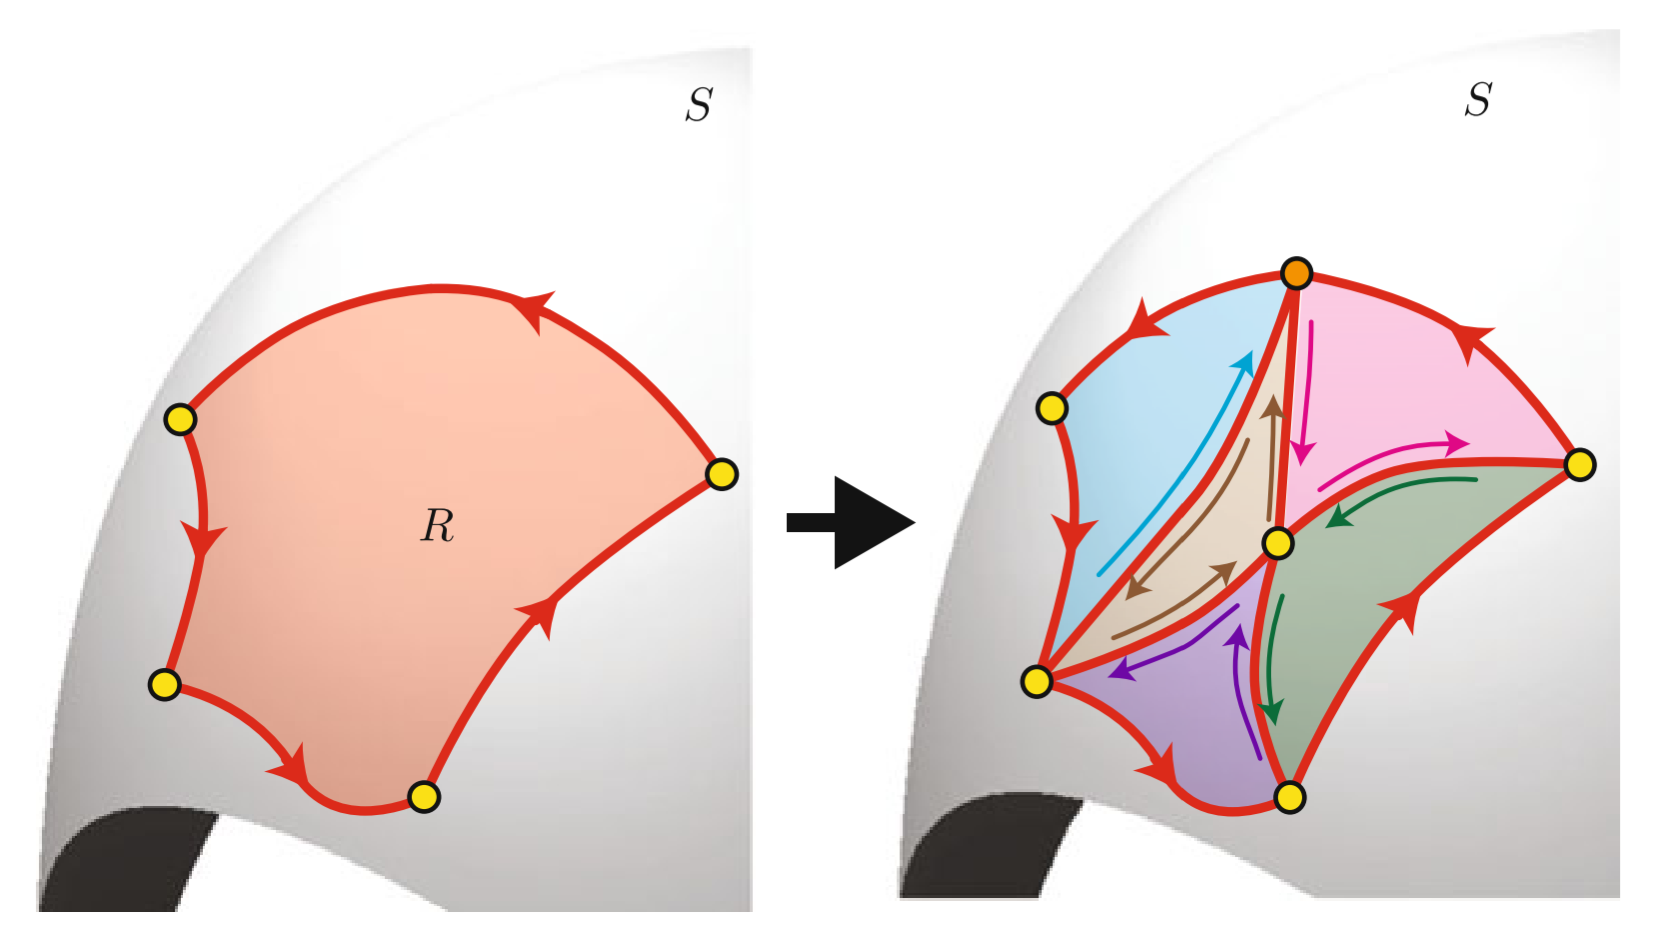
\includegraphics[width=0.5\textwidth]{img/triangulation.png}
	\caption{A triangulation of $R$. Each interior edge receives opposite orientations from the two triangles that share it. Here $\chi(R) = V - E + F = 6 - 10 + 5 = 1$.}
	\label{}
\end{figure}

\begin{theorem}[]\label{}
If $R$ is a regular region of a regular surface $S$, then there exists a triangulation of $R$. Furthermore, every two triangulations of $R$ have the same Euler characteristic.
\end{theorem}

This is a remarkable result. It states that no matter how you ``mesh" a ``nice'' surface, a particular combination of faces, edges, and vertices will always remain constant, and thus contains information that is inherent to the surface.

\begin{remark}[]\label{}
It may be shown that the Euler characteristic is related to the \textbf{genus} of a surface, defined by $\chi = 2 - 2g + b$, where $b$ is the number of boundary components. The genus is related to the number of ``holes" a surface has.
\end{remark}

\begin{definition}[]\label{}
The \textbf{exterior angle} at the junction of two piecewise differentiable curves is the angular difference between the tangent vectors at the junction.
\end{definition}
% \begin{definition}[]\label{}
% Let $\Sigma$ be a surface (possibly with boundary). A \textbf{polygonal triangulation} of $\Sigma$ is a collection of verticies and edges such that
% \begin{enumerate}[i)]
% \item both boundary points of each edge are vertices
% \item each vertex is a boundary for at least one edge
% \item each edge is disjoint from the vertices except at its boundaries
% \item all edges are disjoint from one another except possible at their boundaries
% \item each face is a smooth polygon
% \end{enumerate}
% \end{definition}

% \begin{definition}[]\label{}
% Given a finite polygonal triangulation of $\Sigma$ with $v$ many vertices, $e$ many edges, and $f$ many faces, the \textbf{Euler characteristic} of $\Sigma$, $\chi(\Sigma)$, is the integer $\chi(\Sigma) \defn v - e + f$.
% \end{definition}


% This statement is encapsulated in the following result.
%

\begin{figure}[!htb]
	\centering
	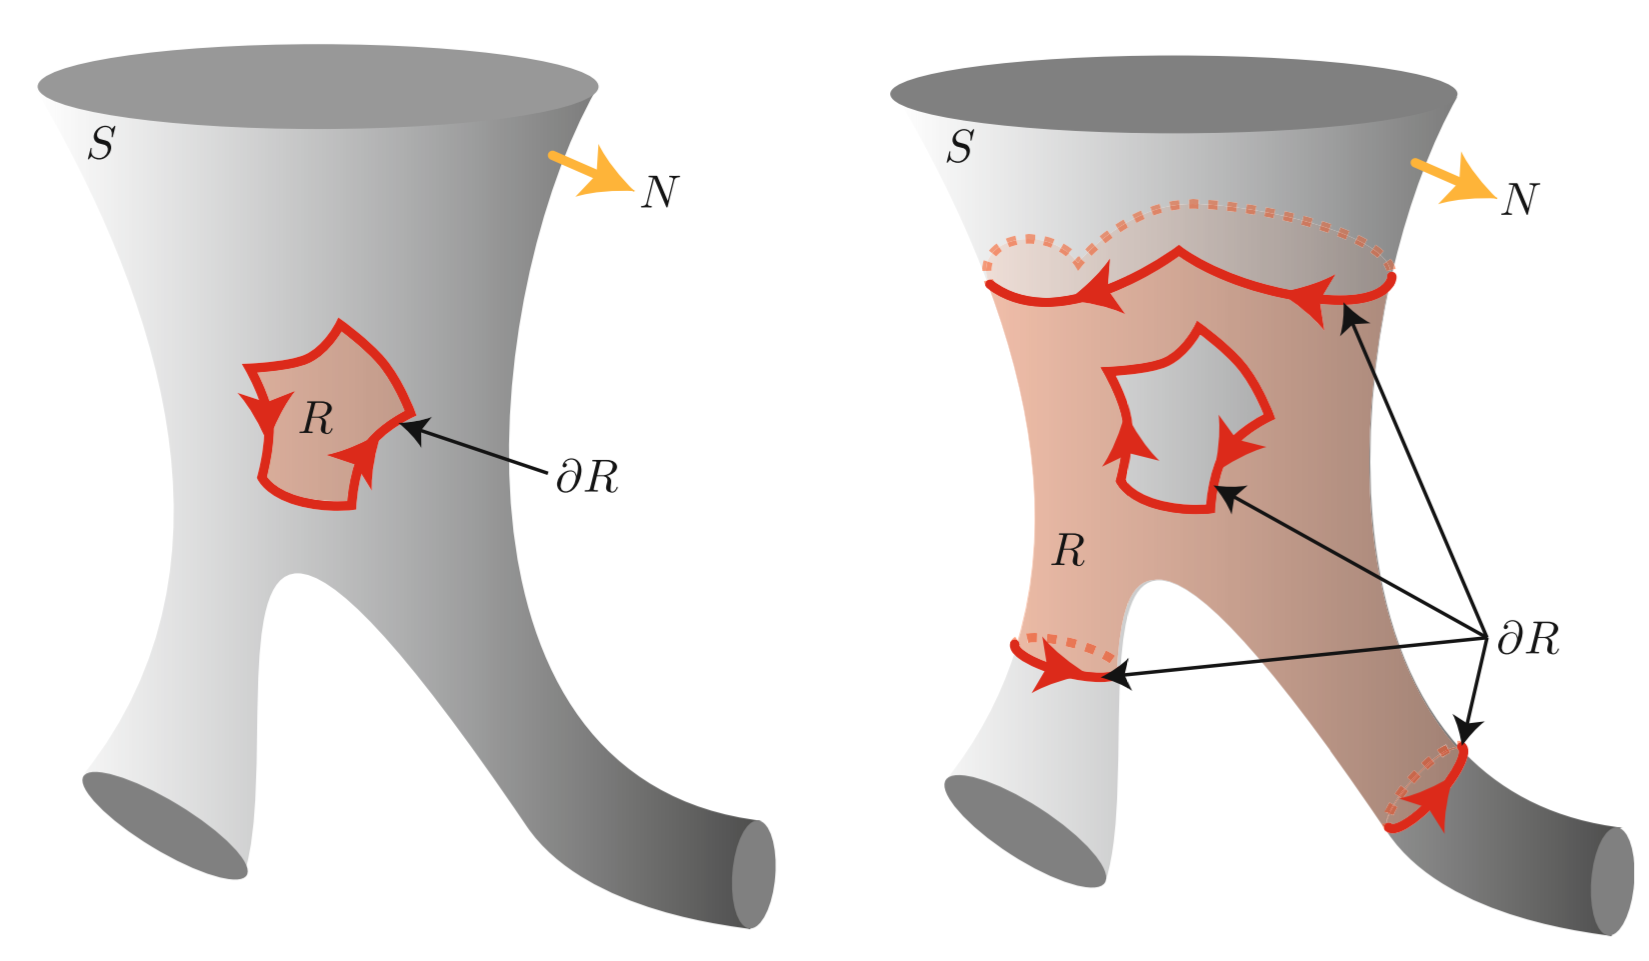
\includegraphics[width=0.5\textwidth]{img/global-gauss-bonnet.png}
	\caption{Example of regular regions with positively oriented boundary components that Gauss-Bonnet may be applied to.}
	\label{fig:gauss-bonnet-global}
\end{figure}

\begin{figure}[!htb]
	\centering
	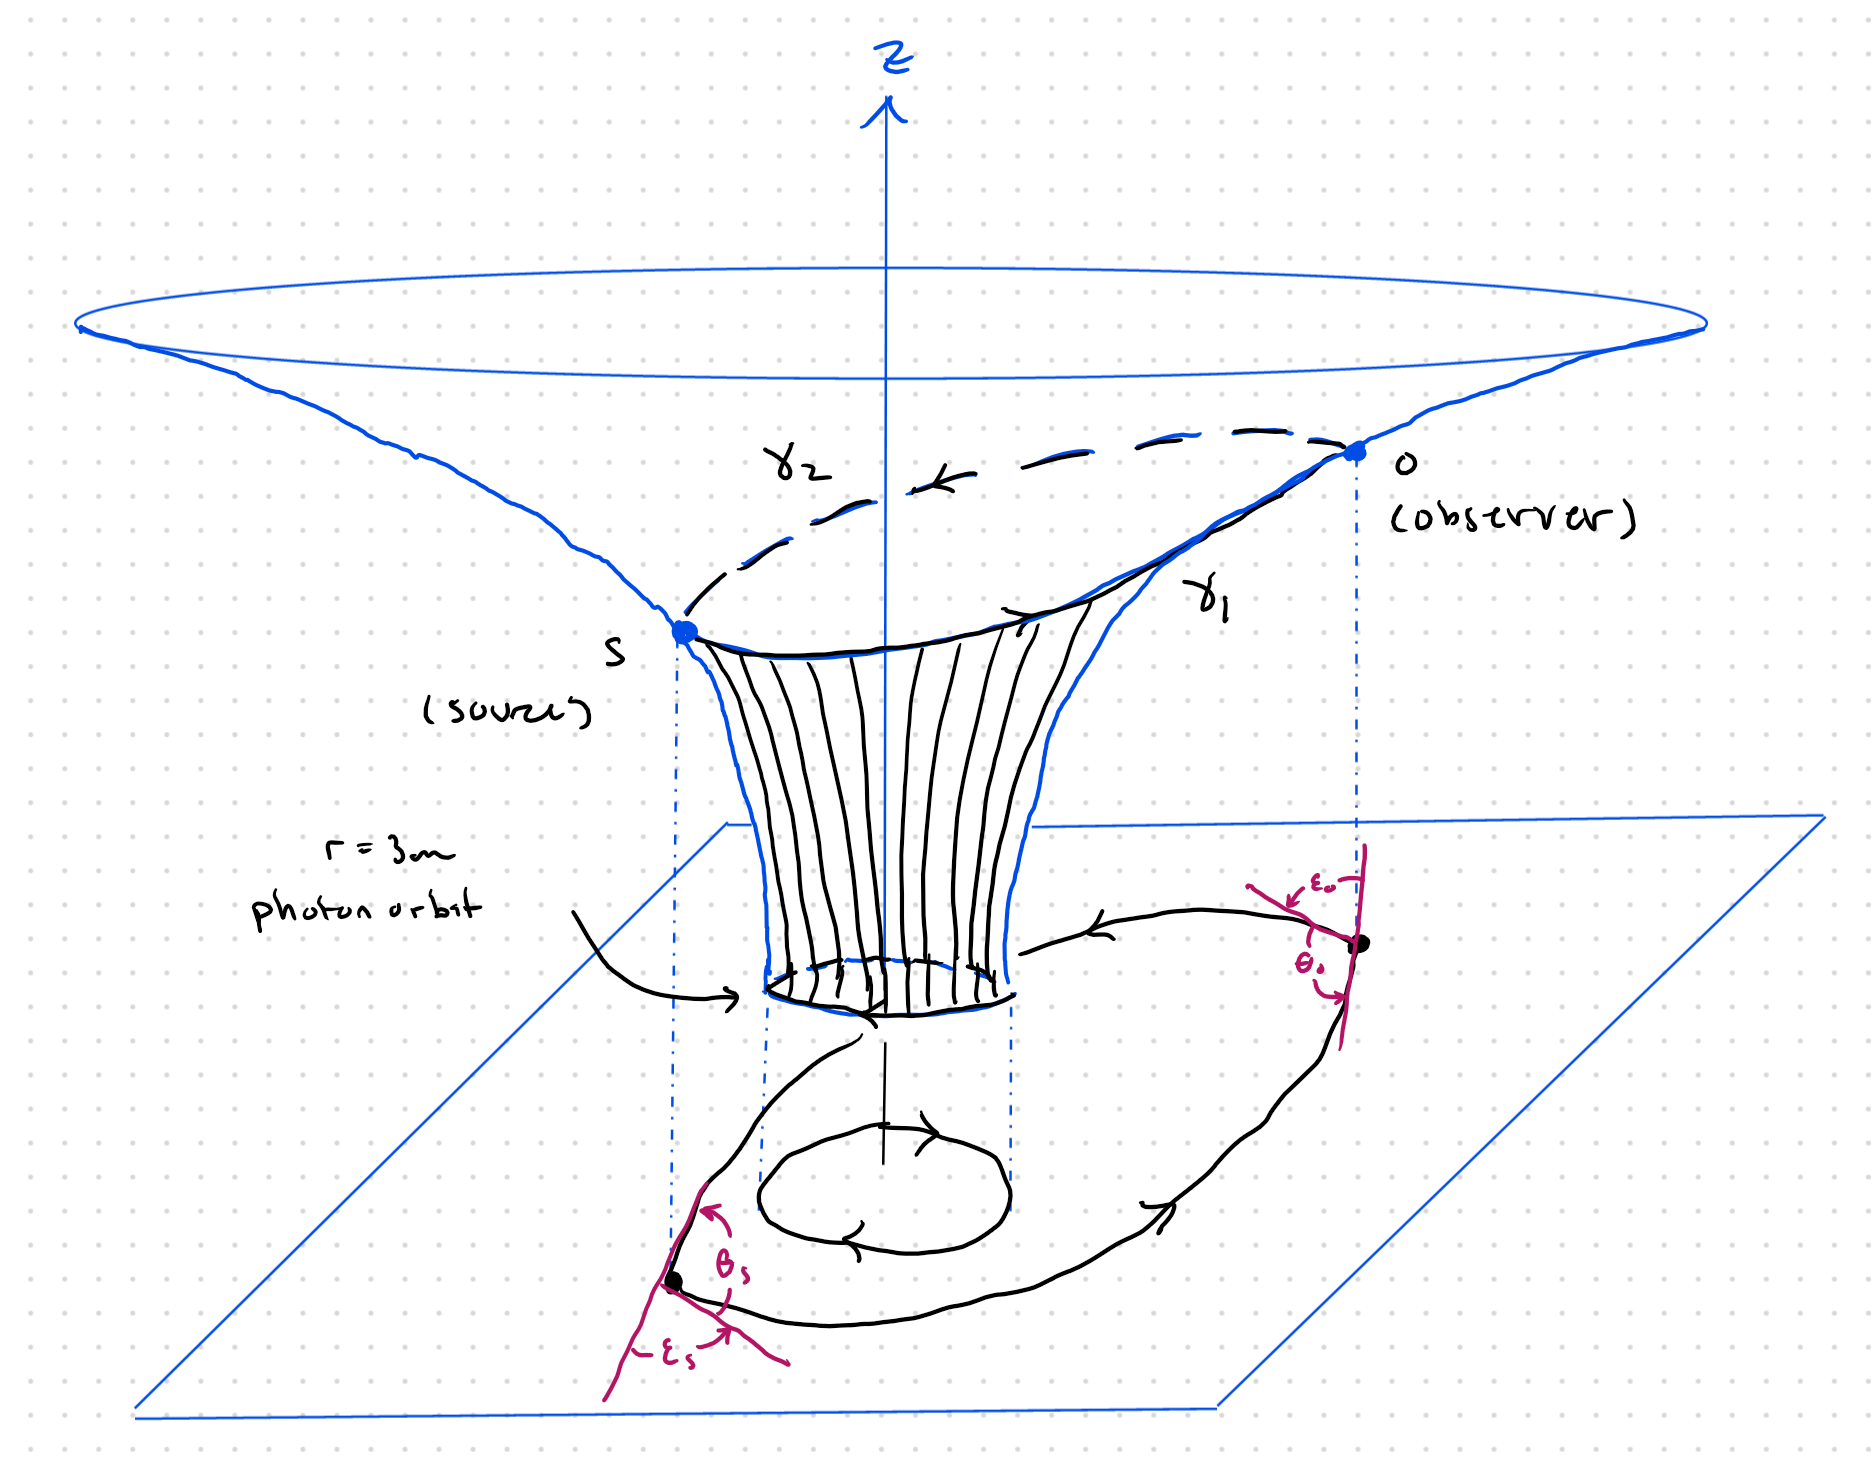
\includegraphics[width=0.65\textwidth]{img/gauss-bonnet-setup.png}
	\caption{We apply the Gauss-Bonnet theorem to the black region. Note that it is bounded on the bottom by the $r=3m$ photon orbit (which is a geodesic), and by two other geodesics $\gamma_1, \gamma_2$.}
	\label{fig:gauss-bonnet-setup}
\end{figure}

\begin{theorem}[Global Gauss-Bonnet]\label{thm:gauss-bonnet}
Let $\Sigma$ be a regular oriented surface with Gaussian curvature $K$, geodesic curvature $k_g$ along $\partial \Sigma = C_1 \cup C_2 \cup \ldots \cup C_i$, where $C_i$ are closed, simple, piecewise and regular curves with exterior angles $\alpha_1, \ldots, \alpha_p$. Then
\begin{equation}\label{eq:gauss-bonnet}
\int_R K dA + \sum_{i=1}^n \int_{C_i} k_g ds + \sum_{i=1}^p \alpha_p = 2 \pi \chi(\Sigma)
\end{equation}
where $\chi(\Sigma)$ is the Euler characteristic of the surface $\Sigma$.
\end{theorem}
Although this result may seem intimidating, the way we use it in practice should be familiar: in particular, its use resembles contour integration and Stokes theorem. That is, we define a region bounded by oriented curves, and relate various quantities on the boundaries with various quantities on the domain. See \cref{fig:gauss-bonnet-global}.



\subsection{Applications to gravitational lensing}
\begin{theorem}[]\label{thm:nontrivial-topology}
Any two geodesics emanating from the same point $s \in \Sigma$ (source) that meet at $o \in \Sigma$ (observer) on a surface with everywhere negative curvature necessarily enclose a region $R$ with nontrivial genus. That is, $g(R) \ge 1$.
\end{theorem}
\begin{proof}
We use the setup described in \cref{fig:gauss-bonnet-setup}. For two geodesics two meet, the enclosed area must have interior angles $\theta_1, \theta_2$ such that $\theta_1 + \theta_2 > 0$. The interior angles are given by $\sum_{i=1}^p \alpha_p = \sum_{i=1}^p(\pi-\theta_i) = p \pi - \sum_{i=1}^p \theta_i$. For our case $p=2$, and \cref{eq:gauss-bonnet} may be simplified to
\begin{align*}
&\int_R K dA + \sum_{i=1}^n \int_{C_i} k_g ds + 2 \pi - \theta_s - \theta_o = 2 \pi \chi(\Sigma) \\
&\implies \theta_s + \theta_o = 2 \pi (1 - \chi) + \int_R K dA + \sum_{i=1}^n \int_{C_i} k_g ds \\
&\implies \theta_s + \theta_o = 2 \pi g + \int_R K dA > 0
\end{align*}
where in the second to last line we've used the fact that the geodesic curvature along all curves forming the boundary is zero (because they are all geodesics).
Therefore $g \ge 1$ is a necessary condition for geodesics to reunite.
\end{proof}
This state of affairs is actually well known, see \cref{fig:geodesics-cylinder}.
\begin{figure}[!htb]
	\centering
	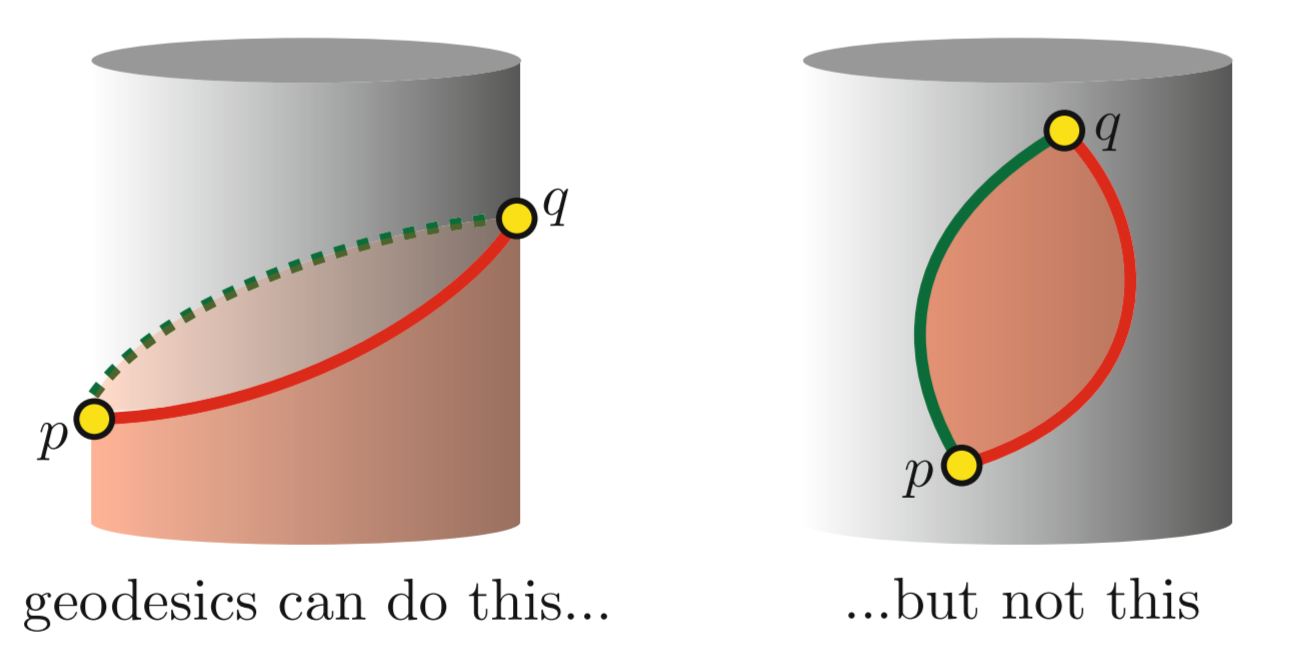
\includegraphics[width=0.5\textwidth]{img/geodesics-on-cylinder.png}
	\caption{How geodesics can rejoin on the cylinder.}
	\label{fig:geodesics-cylinder}
\end{figure}
% \begin{theorem}[Gauss's Theorema Egregium]\label{}
% The gaussian curvature $K$ of a surface $\Sigma$
% \end{theorem}
\section{Conclusion}
The purpose of this note was to show that gravitational lensing has topological origins. To prove this, we introduced the technique of \textit{optical geometry}, which simplifies the study of light rays on Lorentzian manifolds to the study of spatial light rays on a simpler \textit{Fermat metric}. We then applied this technique to the particular case of a \textit{Schwarzschild spacetime}, and showed that the nontrivial topology of the optical geometry was a necessary condition to ensure that gravitational lensing effects occur.

This line of reasoning leads to many deeper results as well. For example, one may calculate an exact deflection angle in terms of the Gaussian curvature, and show that the leading order term agrees with the quasi-Newton approach. More dramatically, one may use results in Morse theory\footnote{Morse theory is an approach that studies functions (so called Morse functions) on a manifold in order to probe the underlying manifold on which they are defined.} to show that only an \textit{odd number of images} may ever be formed due to gravitational lensing \cite{Hasse_2006}.

% \begin{theorem}[Global Gauss Bonnet]\label{}
% Suppose $M$ is a compact two dimensional Riemannian manifold with boundary. Let $K$ be the Gaussian curvature of M, and let $k_g$ be the geodesic curvature on the boundary. Then
% \begin{equation}\label{}
% \int_M K \, dA + \int_{\partial M} k_g \, ds = 2 \pi \xi(M)
% \end{equation}
% where $dA$ is area element, $ds$ is the line element along the boundary, and $\xi(M)$ is the Euler characteristic of $M$.
% \end{theorem}

\bibliographystyle{amsplain}
\bibliography{references}

\end{document}
